%\documentclass{book}%
\documentclass[12pt, fleqn]{book} % Default font size and left-justified equations%% Based on a TeXnicCenter-Template by Gyorgy SZEIDL.
%%%%%%%%%%%%%%%%%%%%%%%%%%%%%%%%%%%%%%%%%%%%%%%%%%%%%%%%%%%%%
%----------------------------------------------------------
%
%
%----------------------------------------------------------
% This is a sample document for the standard LaTeX Book Class
% Class options
%       --  Body text point size:
%                        10pt (default), 11pt, 12pt
%       --  Paper size:  letterpaper (8.5x11 inch, default)
%                        a4paper, a5paper, b5paper,
%                        legalpaper, executivepaper
%       --  Orientation (portrait is the default):
%                        landscape
%       --  Printside:   oneside, twoside (default)
%       --  Quality:     final(default), draft
%       --  Title page:  titlepage, notitlepage
%       --  Columns:     onecolumn (default), twocolumn
%       --  Start chapter on left:
%                        openright(no, default), openany
%       --  Equation numbering (equation numbers on right is the default):
%                        leqno
%       --  Displayed equations (centered is the default):
%                        fleqn (flush left)
%       --  Open bibliography style (closed bibliography is the default):
%                        openbib
% For instance the command
%          \documentclass[a4paper,12pt,reqno]{book}
% ensures that the paper size is a4, fonts are typeset at the size 12p
% and the equation numbers are on the right side.
%

%%%%%%%%%%%%%%%%%%%%%%%%%%%%%%%%%%%%%%%%%
% The Legrand Orange Book
% Structural Definitions File
% Version 2.0 (9/2/15)
%
% Original author:
% Mathias Legrand (legrand.mathias@gmail.com) with modifications by:
% Vel (vel@latextemplates.com)
% 
% This file has been downloaded from:
% http://www.LaTeXTemplates.com
%
% License:
% CC BY-NC-SA 3.0 (http://creativecommons.org/licenses/by-nc-sa/3.0/)
%
%%%%%%%%%%%%%%%%%%%%%%%%%%%%%%%%%%%%%%%%%

%----------------------------------------------------------------------------------------
%	VARIOUS REQUIRED PACKAGES AND CONFIGURATIONS
%----------------------------------------------------------------------------------------

\usepackage[top=3cm,bottom=3cm,left=3cm,right=3cm,headsep=10pt,a4paper]{geometry} % Page margins

\usepackage{graphicx} % Required for including pictures
\graphicspath{{Pictures/}} % Specifies the directory where pictures are stored

\usepackage{lipsum} % Inserts dummy text

\usepackage{tikz} % Required for drawing custom shapes

\usepackage[english]{babel} % English language/hyphenation

\usepackage{enumitem} % Customize lists
\setlist{nolistsep} % Reduce spacing between bullet points and numbered lists

\usepackage{booktabs} % Required for nicer horizontal rules in tables

\usepackage{xcolor} % Required for specifying colors by name
\definecolor{ocre}{RGB}{243,102,25} % Define the orange color used for highlighting throughout the book

%----------------------------------------------------------------------------------------
%	FONTS
%----------------------------------------------------------------------------------------

\usepackage{avant} % Use the Avantgarde font for headings
%\usepackage{times} % Use the Times font for headings
\usepackage{mathptmx} % Use the Adobe Times Roman as the default text font together with math symbols from the Sym­bol, Chancery and Com­puter Modern fonts

\usepackage{microtype} % Slightly tweak font spacing for aesthetics
\usepackage[utf8]{inputenc} % Required for including letters with accents
\usepackage[T1]{fontenc} % Use 8-bit encoding that has 256 glyphs

%----------------------------------------------------------------------------------------
%	BIBLIOGRAPHY AND INDEX
%----------------------------------------------------------------------------------------

\usepackage[style=numeric,citestyle=numeric,sorting=nyt,sortcites=true,autopunct=true,babel=hyphen,hyperref=true,abbreviate=false,backref=true,backend=biber]{biblatex}
\addbibresource{bibliography.bib} % BibTeX bibliography file
\defbibheading{bibempty}{}

\usepackage{calc} % For simpler calculation - used for spacing the index letter headings correctly
\usepackage{makeidx} % Required to make an index
\makeindex % Tells LaTeX to create the files required for indexing

%----------------------------------------------------------------------------------------
%	MAIN TABLE OF CONTENTS
%----------------------------------------------------------------------------------------

\usepackage{titletoc} % Required for manipulating the table of contents

\contentsmargin{0cm} % Removes the default margin

% Part text styling
\titlecontents{part}[0cm]
{\addvspace{20pt}\centering\large\bfseries}
{}
{}
{}

% Chapter text styling
\titlecontents{chapter}[1.25cm] % Indentation
{\addvspace{12pt}\large\sffamily\bfseries} % Spacing and font options for chapters
{\color{ocre!60}\contentslabel[\Large\thecontentslabel]{1.25cm}\color{ocre}} % Chapter number
{\color{ocre}}  
{\color{ocre!60}\normalsize\;\titlerule*[.5pc]{.}\;\thecontentspage} % Page number

% Section text styling
\titlecontents{section}[1.25cm] % Indentation
{\addvspace{3pt}\sffamily\bfseries} % Spacing and font options for sections
{\contentslabel[\thecontentslabel]{1.25cm}} % Section number
{}
{\hfill\color{black}\thecontentspage} % Page number
[]

% Subsection text styling
\titlecontents{subsection}[1.25cm] % Indentation
{\addvspace{1pt}\sffamily\small} % Spacing and font options for subsections
{\contentslabel[\thecontentslabel]{1.25cm}} % Subsection number
{}
{\ \titlerule*[.5pc]{.}\;\thecontentspage} % Page number
[]

% List of figures
\titlecontents{figure}[0em]
{\addvspace{-5pt}\sffamily}
{\thecontentslabel\hspace*{1em}}
{}
{\ \titlerule*[.5pc]{.}\;\thecontentspage}
[]

% List of tables
\titlecontents{table}[0em]
{\addvspace{-5pt}\sffamily}
{\thecontentslabel\hspace*{1em}}
{}
{\ \titlerule*[.5pc]{.}\;\thecontentspage}
[]

%----------------------------------------------------------------------------------------
%	MINI TABLE OF CONTENTS IN PART HEADS
%----------------------------------------------------------------------------------------

% Chapter text styling
\titlecontents{lchapter}[0em] % Indenting
{\addvspace{15pt}\large\sffamily\bfseries} % Spacing and font options for chapters
{\color{ocre}\contentslabel[\Large\thecontentslabel]{1.25cm}\color{ocre}} % Chapter number
{}  
{\color{ocre}\normalsize\sffamily\bfseries\;\titlerule*[.5pc]{.}\;\thecontentspage} % Page number

% Section text styling
\titlecontents{lsection}[0em] % Indenting
{\sffamily\small} % Spacing and font options for sections
{\contentslabel[\thecontentslabel]{1.25cm}} % Section number
{}
{}

% Subsection text styling
\titlecontents{lsubsection}[.5em] % Indentation
{\normalfont\footnotesize\sffamily} % Font settings
{}
{}
{}

%----------------------------------------------------------------------------------------
%	PAGE HEADERS
%----------------------------------------------------------------------------------------

\usepackage{fancyhdr} % Required for header and footer configuration

\pagestyle{fancy}
\renewcommand{\chaptermark}[1]{\markboth{\sffamily\normalsize\bfseries\chaptername\ \thechapter.\ #1}{}} % Chapter text font settings
\renewcommand{\sectionmark}[1]{\markright{\sffamily\normalsize\thesection\hspace{5pt}#1}{}} % Section text font settings
\fancyhf{} \fancyhead[LE,RO]{\sffamily\normalsize\thepage} % Font setting for the page number in the header
\fancyhead[LO]{\rightmark} % Print the nearest section name on the left side of odd pages
\fancyhead[RE]{\leftmark} % Print the current chapter name on the right side of even pages
\renewcommand{\headrulewidth}{0.5pt} % Width of the rule under the header
\addtolength{\headheight}{2.5pt} % Increase the spacing around the header slightly
\renewcommand{\footrulewidth}{0pt} % Removes the rule in the footer
\fancypagestyle{plain}{\fancyhead{}\renewcommand{\headrulewidth}{0pt}} % Style for when a plain pagestyle is specified

% Removes the header from odd empty pages at the end of chapters
\makeatletter
\renewcommand{\cleardoublepage}{
\clearpage\ifodd\c@page\else
\hbox{}
\vspace*{\fill}
\thispagestyle{empty}
\newpage
\fi}

%----------------------------------------------------------------------------------------
%	THEOREM STYLES
%----------------------------------------------------------------------------------------

\usepackage{amsmath,amsfonts,amssymb,amsthm} % For math equations, theorems, symbols, etc

\newcommand{\intoo}[2]{\mathopen{]}#1\,;#2\mathclose{[}}
\newcommand{\ud}{\mathop{\mathrm{{}d}}\mathopen{}}
\newcommand{\intff}[2]{\mathopen{[}#1\,;#2\mathclose{]}}
\newtheorem{notation}{Notation}[chapter]

% Boxed/framed environments
\newtheoremstyle{ocrenumbox}% % Theorem style name
{0pt}% Space above
{0pt}% Space below
{\normalfont}% % Body font
{}% Indent amount
{\small\bf\sffamily\color{ocre}}% % Theorem head font
{\;}% Punctuation after theorem head
{0.25em}% Space after theorem head
{\small\sffamily\color{ocre}\thmname{#1}\nobreakspace\thmnumber{\@ifnotempty{#1}{}\@upn{#2}}% Theorem text (e.g. Theorem 2.1)
\thmnote{\nobreakspace\the\thm@notefont\sffamily\bfseries\color{black}---\nobreakspace#3.}} % Optional theorem note
\renewcommand{\qedsymbol}{$\blacksquare$}% Optional qed square

\newtheoremstyle{blacknumex}% Theorem style name
{5pt}% Space above
{5pt}% Space below
{\normalfont}% Body font
{} % Indent amount
{\small\bf\sffamily}% Theorem head font
{\;}% Punctuation after theorem head
{0.25em}% Space after theorem head
{\small\sffamily{\tiny\ensuremath{\blacksquare}}\nobreakspace\thmname{#1}\nobreakspace\thmnumber{\@ifnotempty{#1}{}\@upn{#2}}% Theorem text (e.g. Theorem 2.1)
\thmnote{\nobreakspace\the\thm@notefont\sffamily\bfseries---\nobreakspace#3.}}% Optional theorem note

\newtheoremstyle{blacknumbox} % Theorem style name
{0pt}% Space above
{0pt}% Space below
{\normalfont}% Body font
{}% Indent amount
{\small\bf\sffamily}% Theorem head font
{\;}% Punctuation after theorem head
{0.25em}% Space after theorem head
{\small\sffamily\thmname{#1}\nobreakspace\thmnumber{\@ifnotempty{#1}{}\@upn{#2}}% Theorem text (e.g. Theorem 2.1)
\thmnote{\nobreakspace\the\thm@notefont\sffamily\bfseries---\nobreakspace#3.}}% Optional theorem note

% Non-boxed/non-framed environments
\newtheoremstyle{ocrenum}% % Theorem style name
{5pt}% Space above
{5pt}% Space below
{\normalfont}% % Body font
{}% Indent amount
{\small\bf\sffamily\color{ocre}}% % Theorem head font
{\;}% Punctuation after theorem head
{0.25em}% Space after theorem head
{\small\sffamily\color{ocre}\thmname{#1}\nobreakspace\thmnumber{\@ifnotempty{#1}{}\@upn{#2}}% Theorem text (e.g. Theorem 2.1)
\thmnote{\nobreakspace\the\thm@notefont\sffamily\bfseries\color{black}---\nobreakspace#3.}} % Optional theorem note
\renewcommand{\qedsymbol}{$\blacksquare$}% Optional qed square
\makeatother

% Defines the theorem text style for each type of theorem to one of the three styles above
\newcounter{dummy} 
\numberwithin{dummy}{section}
\theoremstyle{ocrenumbox}
\newtheorem{theoremeT}[dummy]{Theorem}
\newtheorem{problem}{Problem}[chapter]
\newtheorem{exerciseT}{Exercise}[chapter]
\theoremstyle{blacknumex}
\newtheorem{exampleT}{Example}[chapter]
\theoremstyle{blacknumbox}
\newtheorem{vocabulary}{Vocabulary}[chapter]
\newtheorem{definitionT}{Definition}[section]
\newtheorem{corollaryT}[dummy]{Corollary}
\theoremstyle{ocrenum}
\newtheorem{proposition}[dummy]{Proposition}

%----------------------------------------------------------------------------------------
%	DEFINITION OF COLORED BOXES
%----------------------------------------------------------------------------------------

\RequirePackage[framemethod=default]{mdframed} % Required for creating the theorem, definition, exercise and corollary boxes

% Theorem box
\newmdenv[skipabove=7pt,
skipbelow=7pt,
backgroundcolor=black!5,
linecolor=ocre,
innerleftmargin=5pt,
innerrightmargin=5pt,
innertopmargin=5pt,
leftmargin=0cm,
rightmargin=0cm,
innerbottommargin=5pt]{tBox}

% Exercise box	  
\newmdenv[skipabove=7pt,
skipbelow=7pt,
rightline=false,
leftline=true,
topline=false,
bottomline=false,
backgroundcolor=ocre!10,
linecolor=ocre,
innerleftmargin=5pt,
innerrightmargin=5pt,
innertopmargin=5pt,
innerbottommargin=5pt,
leftmargin=0cm,
rightmargin=0cm,
linewidth=4pt]{eBox}	

% Definition box
\newmdenv[skipabove=7pt,
skipbelow=7pt,
rightline=false,
leftline=true,
topline=false,
bottomline=false,
linecolor=ocre,
innerleftmargin=5pt,
innerrightmargin=5pt,
innertopmargin=0pt,
leftmargin=0cm,
rightmargin=0cm,
linewidth=4pt,
innerbottommargin=0pt]{dBox}	

% Corollary box
\newmdenv[skipabove=7pt,
skipbelow=7pt,
rightline=false,
leftline=true,
topline=false,
bottomline=false,
linecolor=gray,
backgroundcolor=black!5,
innerleftmargin=5pt,
innerrightmargin=5pt,
innertopmargin=5pt,
leftmargin=0cm,
rightmargin=0cm,
linewidth=4pt,
innerbottommargin=5pt]{cBox}

% Creates an environment for each type of theorem and assigns it a theorem text style from the "Theorem Styles" section above and a colored box from above
\newenvironment{theorem}{\begin{tBox}\begin{theoremeT}}{\end{theoremeT}\end{tBox}}
\newenvironment{exercise}{\begin{eBox}\begin{exerciseT}}{\hfill{\color{ocre}\tiny\ensuremath{\blacksquare}}\end{exerciseT}\end{eBox}}				  
\newenvironment{definition}{\begin{dBox}\begin{definitionT}}{\end{definitionT}\end{dBox}}	
\newenvironment{example}{\begin{exampleT}}{\hfill{\tiny\ensuremath{\blacksquare}}\end{exampleT}}		
\newenvironment{corollary}{\begin{cBox}\begin{corollaryT}}{\end{corollaryT}\end{cBox}}	

%----------------------------------------------------------------------------------------
%	REMARK ENVIRONMENT
%----------------------------------------------------------------------------------------

\newenvironment{remark}{\par\vspace{10pt}\small % Vertical white space above the remark and smaller font size
\begin{list}{}{
\leftmargin=35pt % Indentation on the left
\rightmargin=25pt}\item\ignorespaces % Indentation on the right
\makebox[-2.5pt]{\begin{tikzpicture}[overlay]
\node[draw=ocre!60,line width=1pt,circle,fill=ocre!25,font=\sffamily\bfseries,inner sep=2pt,outer sep=0pt] at (-15pt,0pt){\textcolor{ocre}{R}};\end{tikzpicture}} % Orange R in a circle
\advance\baselineskip -1pt}{\end{list}\vskip5pt} % Tighter line spacing and white space after remark

%----------------------------------------------------------------------------------------
%	SECTION NUMBERING IN THE MARGIN
%----------------------------------------------------------------------------------------

\makeatletter
\renewcommand{\@seccntformat}[1]{\llap{\textcolor{ocre}{\csname the#1\endcsname}\hspace{1em}}}                    
\renewcommand{\section}{\@startsection{section}{1}{\z@}
{-4ex \@plus -1ex \@minus -.4ex}
{1ex \@plus.2ex }
{\normalfont\large\sffamily\bfseries}}
\renewcommand{\subsection}{\@startsection {subsection}{2}{\z@}
{-3ex \@plus -0.1ex \@minus -.4ex}
{0.5ex \@plus.2ex }
{\normalfont\sffamily\bfseries}}
\renewcommand{\subsubsection}{\@startsection {subsubsection}{3}{\z@}
{-2ex \@plus -0.1ex \@minus -.2ex}
{.2ex \@plus.2ex }
{\normalfont\small\sffamily\bfseries}}                        
\renewcommand\paragraph{\@startsection{paragraph}{4}{\z@}
{-2ex \@plus-.2ex \@minus .2ex}
{.1ex}
{\normalfont\small\sffamily\bfseries}}

%----------------------------------------------------------------------------------------
%	PART HEADINGS
%----------------------------------------------------------------------------------------

% numbered part in the table of contents
\newcommand{\@mypartnumtocformat}[2]{%
\setlength\fboxsep{0pt}%
\noindent\colorbox{ocre!20}{\strut\parbox[c][.7cm]{\ecart}{\color{ocre!70}\Large\sffamily\bfseries\centering#1}}\hskip\esp\colorbox{ocre!40}{\strut\parbox[c][.7cm]{\linewidth-\ecart-\esp}{\Large\sffamily\centering#2}}}%
%%%%%%%%%%%%%%%%%%%%%%%%%%%%%%%%%%
% unnumbered part in the table of contents
\newcommand{\@myparttocformat}[1]{%
\setlength\fboxsep{0pt}%
\noindent\colorbox{ocre!40}{\strut\parbox[c][.7cm]{\linewidth}{\Large\sffamily\centering#1}}}%
%%%%%%%%%%%%%%%%%%%%%%%%%%%%%%%%%%
\newlength\esp
\setlength\esp{4pt}
\newlength\ecart
\setlength\ecart{1.2cm-\esp}
\newcommand{\thepartimage}{}%
\newcommand{\partimage}[1]{\renewcommand{\thepartimage}{#1}}%
\def\@part[#1]#2{%
\ifnum \c@secnumdepth >-2\relax%
\refstepcounter{part}%
\addcontentsline{toc}{part}{\texorpdfstring{\protect\@mypartnumtocformat{\thepart}{#1}}{\partname~\thepart\ ---\ #1}}
\else%
\addcontentsline{toc}{part}{\texorpdfstring{\protect\@myparttocformat{#1}}{#1}}%
\fi%
\startcontents%
\markboth{}{}%
{\thispagestyle{empty}%
\begin{tikzpicture}[remember picture,overlay]%
\node at (current page.north west){\begin{tikzpicture}[remember picture,overlay]%	
\fill[ocre!20](0cm,0cm) rectangle (\paperwidth,-\paperheight);
\node[anchor=north] at (4cm,-3.25cm){\color{ocre!40}\fontsize{220}{100}\sffamily\bfseries\thepart}; 
\node[anchor=south east] at (\paperwidth-1cm,-\paperheight+1cm){\parbox[t][][t]{8.5cm}{
\printcontents{l}{0}{\setcounter{tocdepth}{1}}%
}};
\node[anchor=north east] at (\paperwidth-1.5cm,-3.25cm){\parbox[t][][t]{15cm}{\strut\raggedleft\color{white}\fontsize{30}{30}\sffamily\bfseries#2}};
\end{tikzpicture}};
\end{tikzpicture}}%
\@endpart}
\def\@spart#1{%
\startcontents%
\phantomsection
{\thispagestyle{empty}%
\begin{tikzpicture}[remember picture,overlay]%
\node at (current page.north west){\begin{tikzpicture}[remember picture,overlay]%	
\fill[ocre!20](0cm,0cm) rectangle (\paperwidth,-\paperheight);
\node[anchor=north east] at (\paperwidth-1.5cm,-3.25cm){\parbox[t][][t]{15cm}{\strut\raggedleft\color{white}\fontsize{30}{30}\sffamily\bfseries#1}};
\end{tikzpicture}};
\end{tikzpicture}}
\addcontentsline{toc}{part}{\texorpdfstring{%
\setlength\fboxsep{0pt}%
\noindent\protect\colorbox{ocre!40}{\strut\protect\parbox[c][.7cm]{\linewidth}{\Large\sffamily\protect\centering #1\quad\mbox{}}}}{#1}}%
\@endpart}
\def\@endpart{\vfil\newpage
\if@twoside
\if@openright
\null
\thispagestyle{empty}%
\newpage
\fi
\fi
\if@tempswa
\twocolumn
\fi}

%----------------------------------------------------------------------------------------
%	CHAPTER HEADINGS
%----------------------------------------------------------------------------------------

% A switch to conditionally include a picture, implemented by  Christian Hupfer
\newif\ifusechapterimage
\usechapterimagetrue
\newcommand{\thechapterimage}{}%
\newcommand{\chapterimage}[1]{\ifusechapterimage\renewcommand{\thechapterimage}{#1}\fi}%
\newcommand{\autodot}{.}
\def\@makechapterhead#1{%
{\parindent \z@ \raggedright \normalfont
\ifnum \c@secnumdepth >\m@ne
\if@mainmatter
\begin{tikzpicture}[remember picture,overlay]
\node at (current page.north west)
{\begin{tikzpicture}[remember picture,overlay]
\node[anchor=north west,inner sep=0pt] at (0,0) {\ifusechapterimage\includegraphics[width=\paperwidth]{\thechapterimage}\fi};
\draw[anchor=west] (\Gm@lmargin,-9cm) node [line width=2pt,rounded corners=15pt,draw=ocre,fill=white,fill opacity=0.5,inner sep=15pt]{\strut\makebox[22cm]{}};
\draw[anchor=west] (\Gm@lmargin+.3cm,-9cm) node {\huge\sffamily\bfseries\color{black}\thechapter\autodot~#1\strut};
\end{tikzpicture}};
\end{tikzpicture}
\else
\begin{tikzpicture}[remember picture,overlay]
\node at (current page.north west)
{\begin{tikzpicture}[remember picture,overlay]
\node[anchor=north west,inner sep=0pt] at (0,0) {\ifusechapterimage\includegraphics[width=\paperwidth]{\thechapterimage}\fi};
\draw[anchor=west] (\Gm@lmargin,-9cm) node [line width=2pt,rounded corners=15pt,draw=ocre,fill=white,fill opacity=0.5,inner sep=15pt]{\strut\makebox[22cm]{}};
\draw[anchor=west] (\Gm@lmargin+.3cm,-9cm) node {\huge\sffamily\bfseries\color{black}#1\strut};
\end{tikzpicture}};
\end{tikzpicture}
\fi\fi\par\vspace*{270\p@}}}

%-------------------------------------------

\def\@makeschapterhead#1{%
\begin{tikzpicture}[remember picture,overlay]
\node at (current page.north west)
{\begin{tikzpicture}[remember picture,overlay]
\node[anchor=north west,inner sep=0pt] at (0,0) {\ifusechapterimage\includegraphics[width=\paperwidth]{\thechapterimage}\fi};
\draw[anchor=west] (\Gm@lmargin,-9cm) node [line width=2pt,rounded corners=15pt,draw=ocre,fill=white,fill opacity=0.5,inner sep=15pt]{\strut\makebox[22cm]{}};
\draw[anchor=west] (\Gm@lmargin+.3cm,-9cm) node {\huge\sffamily\bfseries\color{black}#1\strut};
\end{tikzpicture}};
\end{tikzpicture}
\par\vspace*{270\p@}}
\makeatother

%----------------------------------------------------------------------------------------
%	HYPERLINKS IN THE DOCUMENTS
%----------------------------------------------------------------------------------------

\usepackage{hyperref}
\hypersetup{hidelinks,backref=true,pagebackref=true,hyperindex=true,colorlinks=false,breaklinks=true,urlcolor= ocre,bookmarks=true,bookmarksopen=false,pdftitle={Title},pdfauthor={Author}}
\usepackage{bookmark}
\bookmarksetup{
open,
numbered,
addtohook={%
\ifnum\bookmarkget{level}=0 % chapter
\bookmarksetup{bold}%
\fi
\ifnum\bookmarkget{level}=-1 % part
\bookmarksetup{color=ocre,bold}%
\fi
}
}
 % Insert the commands.tex file which contains the majority of the structure behind the template


% FROM THINK LIKE ACOMPUTER SCIENTIST 
\usepackage{epsfig}
\usepackage{makeidx}
\usepackage{url}
\usepackage{amsmath, amsthm, amssymb}
\pssilent

% the following are some commands that appear in the Python version.
% we can use them to adjust some things later, but for now they are
% all blanked out.

\newcommand{\beforefig}{}
\newcommand{\afterfig}{}

\newcommand{\beforeverb}{}
\newcommand{\afterverb}{}

\newcommand{\adjustpage}[1]{}

\newcommand{\clearemptydoublepage}{\cleardoublepage}
\newcommand{\blankpage}{\vspace*{1in}\newpage}

\newtheorem{ex}{Exercise}[chapter]

% END FROM THINK LIKE ACOMPUTER SCIENTIST

\begin{document}

%----------------------------------------------------------------------------------------
%	TITLE PAGE
%----------------------------------------------------------------------------------------

%----------------------------------------------------------------------------------------
%	TITLE PAGE
%----------------------------------------------------------------------------------------

\begingroup
\thispagestyle{empty}
\begin{tikzpicture}[remember picture,overlay]
\node[inner sep=0pt] (background) at (current page.center) {\includegraphics[width=\paperwidth]{background}};
\draw (current page.center) node [fill=ocre!30!white,fill opacity=0.6,text opacity=1,inner sep=1cm]{\Huge\centering\bfseries\sffamily\parbox[c][][t]{\paperwidth}{\centering Theory and Practice of Programming\\[15pt] % Book title
		{\Large An introduction to Python and Computational Thinking}\\[20pt] % Subtitle
		{\huge Dr. Lilian Blot}}}; % Author name
\end{tikzpicture}
\vfill
\endgroup


%----------------------------------------------------------------------------------------
%	COPYRIGHT PAGE
%----------------------------------------------------------------------------------------

\newpage
~\vfill
\thispagestyle{empty}

\noindent Copyright \copyright\ 2018 Lilian Blot\\ % Copyright notice

%\noindent \textsc{Published by Publisher}\\ % Publisher
%
%\noindent \textsc{book-website.com}\\ % URL

\noindent Licensed under the Creative Commons Attribution-NonCommercial 3.0 Unported License (the ``License''). You may not use this file except in compliance with the License. You may obtain a copy of the License at \url{http://creativecommons.org/licenses/by-nc/3.0}. Unless required by applicable law or agreed to in writing, software distributed under the License is distributed on an \textsc{``as is'' basis, without warranties or conditions of any kind}, either express or implied. See the License for the specific language governing permissions and limitations under the License.\\ % License information

%\noindent \textit{First printing, March 2013} % Printing/edition date

%----------------------------------------------------------------------------------------
%	TABLE OF CONTENTS
%----------------------------------------------------------------------------------------

%\usechapterimagefalse % If you don't want to include a chapter image, use this to toggle images off - it can be enabled later with \usechapterimagetrue

\chapterimage{chapter_head_1.pdf} % Table of contents heading image

\pagestyle{empty} % No headers

\tableofcontents % Print the table of contents itself

\cleardoublepage % Forces the first chapter to start on an odd page so it's on the right

\pagestyle{fancy} % Print headers again


%\mainmatter

\part{Part I}

\chapterimage{chapter_head_1.pdf} % Chapter heading image
\chapter{The way of the program}

The goal of this book is to teach you to think like a
computer scientist.  This way of thinking combines some of the best features
of mathematics, engineering, and natural science.  Like mathematicians,
computer scientists use formal languages to denote ideas (specifically
computations).  Like engineers, they design things, assembling components
into systems and evaluating tradeoffs among alternatives.  Like scientists,
they observe the behavior of complex systems, form hypotheses, and test
predictions.

\index{problem solving}

The single most important skill for a computer scientist is {\bf
	problem solving}.  Problem solving means the ability to formulate
problems, think creatively about solutions, and express a solution clearly
and accurately.  As it turns out, the process of learning to program is an
excellent opportunity to practice problem-solving skills.  That's why
this chapter is called, ``The way of the program.''

On one level, you will be learning to program, a useful
skill by itself.  On another level, you will use programming as a means to
an end.  As we go along, that end will become clearer.


\section{The Python programming language}
\index{programming language}
\index{language!programming}

The programming language you will learn is Python. Python is
an example of a {\bf high-level language}; other high-level languages
you might have heard of are C++, C\#, VB, JavaScript, and Java.

There are also {\bf low-level languages}, sometimes referred to as ``machine
languages'' or ``assembly languages.''  Loosely speaking, computers
can only execute programs written in low-level languages.  So
programs written in a high-level language have to be processed before
they can run.  This extra processing takes some time, which is a small
disadvantage of high-level languages.

\index{portability}
\index{high-level language}
\index{low-level language}
\index{language!high-level}
\index{language!low-level}

The advantages are enormous.  First, it is much easier for a human to program
in a high-level language.  Programs written in a high-level language
take less time to write, they are shorter and easier to read, and they
are more likely to be correct.  Second, high-level languages are {\bf
	portable}, meaning that they can run on different kinds of computers
with few or no modifications.  Low-level programs can run on only one
kind of computer and have to be rewritten to run on another.
Due to these advantages, almost all programs are written in high-level
languages.  Low-level languages are used only for a few specialized
applications.

\index{compile}
\index{interpret}

Two kinds of programs process high-level languages
into low-level languages: {\bf interpreters} and {\bf compilers}.
An interpreter reads a high-level program and executes it, meaning that it
does what the program says.  It processes the program a little at a time,
alternately reading lines and performing computations.


%MUST INCLUDE THE FIGURE HERE

\beforefig
\centerline{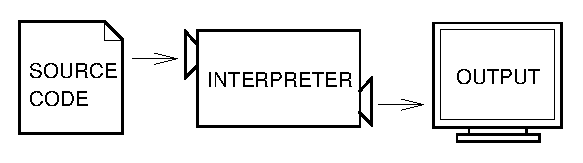
\includegraphics[height=0.77in]{figs/interpret.eps}}
\afterfig

\index{source code}
\index{object code}
\index{executable}

A compiler reads the program and translates it completely before the
program starts running.  In this context, the high-level program is
called the {\bf source code}, and the translated program is called the
{\bf object code} or the {\bf executable}.  Once a program is
compiled, you can execute it repeatedly without further translation.

\beforefig
\centerline{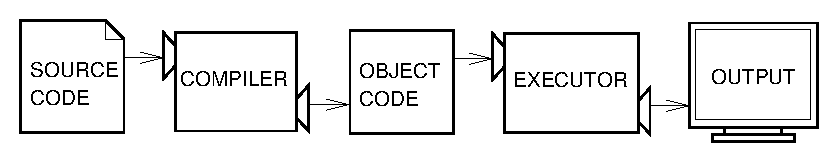
\includegraphics[height=0.77in]{figs/compile.eps}}
\afterfig

Python is considered an interpreted language because Python programs
are executed by an interpreter.  There are two ways to use the
interpreter: {\bf interactive mode} and {\bf script mode}. In
interactive mode, you type Python programs and the interpreter prints
the result:

\index{interactive mode}
\index{script mode}

\beforeverb
\begin{verbatim}
>>> 1 + 1
2
\end{verbatim}
\afterverb
%
The chevron, verb|>>>|, is the
{\bf prompt} the interpreter uses to indicate that it is ready.  If
you type {\tt 1 + 1}, the interpreter replies {\tt 2}.

\index{prompt}

Alternatively, you can store code in a file and use the interpreter to
execute the contents of the file, which is called a {\bf script}.  By
convention, Python scripts have names that end with {\tt .py}.
\index{script}
To execute the script, you have to tell the interpreter the name of
the file. In a Windows command shell, you would type {\tt python
	dinsdale.py}.  In other development environments, the details of
executing scripts are different.  You can find instructions for
your environment at the Python website \url{python.org}.

\index{testing!interactive mode}

Working in interactive mode is convenient for testing small pieces of
code because you can type and execute them immediately.  But for
anything more than a few lines, you should save your code
as a script so you can modify and execute it in the future.


\section{What is a program?}

A {\bf program} is a sequence of instructions that specifies how to
perform a computation.  The computation might be something
mathematical, such as solving a system of equations or finding the
roots of a polynomial, but it can also be a symbolic computation, such
as searching and replacing text in a document or (strangely enough)
compiling a program.

\index{program}

The details look different in different languages, but a few basic
instructions appear in just about every language:

\begin{description}
	
	\item[input:] Get data from the keyboard, a file, or some
	other device.
	
	\item[output:] Display data on the screen or send data to a
	file or other device.
	
	\item[math:] Perform basic mathematical operations like addition and
	multiplication.
	
	\item[conditional execution:] Check for certain conditions and
	execute the appropriate sequence of statements.
	
	\item[repetition:] Perform some action repeatedly, usually with
	some variation.
	
\end{description}

Believe it or not, that's pretty much all there is to it.  Every
program you've ever used, no matter how complicated, is made up of
instructions that look pretty much like these.  So you can think of
programming as the process of breaking a large, complex task
into smaller and smaller subtasks until the subtasks are
simple enough to be performed with one of these basic instructions.
\index{algorithm}
That may be a little vague, but we will come back to this topic
when we talk about {\bf algorithms}.

\section{What is debugging?}
\index{debugging}
\index{bug}

Programming is error-prone.  For whimsical reasons, programming errors
are called {\bf bugs} and the process of tracking them down is called
{\bf debugging}.
\index{debugging}
\index{bug}
Three kinds of errors can occur in a program: syntax errors, runtime 
errors, and semantic errors. It is useful
to distinguish between them in order to track them down more quickly.

\subsection{Syntax errors}
\index{syntax error}
\index{error!syntax}
\index{error message}

Python can only execute a program if the syntax is
correct; otherwise, the interpreter displays an error message.
{\bf Syntax} refers to the structure of a program and the rules about
that structure. \index{syntax} 
For example, parentheses have to come in matching pairs, so
{\tt (1 + 2)} is legal, but {\tt 1 + 2)} is a {\bf syntax error}.

\index{parentheses!matching}
\index{syntax}
\index{cummings, e. e.}

In English readers can tolerate most syntax errors, 
Python is not so forgiving.  If there is a single syntax error
anywhere in your program, Python will display an error message and quit,
and you will not be able to run your program. During the first few
weeks of your programming career, you will probably spend a lot of
time tracking down syntax errors.  As you gain experience, you will
make fewer errors and find them faster.

\subsection{Runtime errors}
\label{runtime}
\index{runtime error}
\index{error!runtime}
\index{exception}
\index{safe language}
\index{language!safe}

The second type of error is a runtime error, so called because the
error does not appear until after the program has started running.
These errors are also called {\bf exceptions} because they usually
indicate that something exceptional (and bad) has happened.
Runtime errors are rare in the simple programs you will see in the
first few chapters, so it might be a while before you encounter one.


\subsection{Semantic errors}
\index{semantics}
\index{semantic error}
\index{error!semantic}
\index{error message}

The third type of error is the {\bf semantic error}.  If there is a
semantic error in your program, it will run successfully in the sense
that the computer will not generate any error messages, but it will
not do the right thing.  It will do something else.  Specifically, it
will do what you told it to do.
The problem is that the program you wrote is not the program you
wanted to write.  The meaning of the program (its semantics) is wrong.
Identifying semantic errors can be tricky because it requires you to work
backward by looking at the output of the program and trying to figure
out what it is doing.

\subsection{Experimental debugging}

One of the most important skills you will acquire is debugging.
Although it can be frustrating, debugging is one of the most
intellectually rich, challenging, and interesting parts of
programming.

\index{experimental debugging}
\index{debugging!experimental}

In some ways, debugging is like detective work.  You are confronted
with clues, and you have to infer the processes and events that led
to the results you see.
Debugging is also like an experimental science.  Once you have an idea
about what is going wrong, you modify your program and try again.  If
your hypothesis was correct, then you can predict the result of the
modification, and you take a step closer to a working program.  If
your hypothesis was wrong, you have to come up with a new one.  As
Sherlock Holmes pointed out~\parencite{doyle2010sign}, ``When you have eliminated the
impossible, whatever remains, however improbable, must be the truth.''


For some people, programming and debugging are the same thing.  That
is, programming is the process of gradually debugging a program until
it does what you want.  The idea is that you should start with a
program that does {\em something} and make small modifications,
debugging them as you go, so that you always have a working program.

For example, Linux is an operating system that contains thousands of
lines of code, but it started out as a simple program Linus Torvalds
used to explore the Intel 80386 chip.  According to Larry Greenfield,
``One of Linus's earlier projects was a program that would switch
between printing AAAA and BBBB.  This later evolved to Linux.''
({\em The Linux Users' Guide} Beta Version 1).

\index{Linux}

Later chapters will make more suggestions about debugging and other
programming practices.

\section{Formal and natural languages}
\index{formal language}
\index{natural language}
\index{language!formal}
\index{language!natural}

\begin{definition}[Natural languages] are the languages people speak,
such as English, Spanish, and French.  They were not designed
by people (although people try to impose some order on them);
they evolved naturally.
\end{definition}

\begin{definition}[Formal languages] are languages that are designed by people for
specific applications.  For example, the notation that mathematicians
use is a formal language that is particularly good at denoting
relationships among numbers and symbols.  Chemists use a formal
language to represent the chemical structure of molecules.  And
most importantly:
\end{definition}

\begin{quote}
	{\bf Programming languages are formal languages that have been
		designed to express computations.}
\end{quote}

Formal languages tend to have strict rules about syntax.  For example,
$3 + 3 = 6$ is a syntactically correct mathematical statement, but 
$3 + = 6 \mbox{\pounds} 3$ is not. 
Syntax rules come in two flavors, pertaining to {\bf tokens} and
structure.  Tokens are the basic elements of the language, such as
words, numbers, operators.  One of the problems with $3 +
= 3 \mbox{\pounds} 6$ is that $\pounds$ is not a legal token in mathematics.

\index{token}
\index{structure}

The second type of syntax error pertains to the structure of a
statement; that is, the way the tokens are arranged.  The statement $3
+ = 6 - 3$ is illegal because even though $+$ and $=$ are
legal tokens, you can't have one right after the other.

When you read a sentence in English or a statement in a formal
language, you have to figure out what the structure of the sentence is
(although in a natural language you do this subconsciously).  This
process is called {\bf parsing}.

\index{parse}

For example, when you hear the sentence, ``The penny dropped,'' you
understand that ``the penny'' is the subject and ``dropped'' is the
predicate.  Once you have parsed a sentence, you can figure out what it
means, or the semantics of the sentence.  Assuming that you know
what a penny is and what it means to drop, you will understand the
general implication of this sentence.

Although formal and natural languages have many features in
common---tokens, structure, syntax, and semantics---there are some
important differences:

\index{ambiguity}
\index{redundancy}
\index{literalness}

\begin{description}
	
	\item[ambiguity:] Natural languages are full of ambiguity, which
	people deal with by using contextual clues and other information.
	Formal languages are designed to be nearly or completely unambiguous,
	which means that any statement has exactly one meaning,
	regardless of context.
	
	\item[redundancy:] In order to make up for ambiguity and reduce
	misunderstandings, natural languages employ lots of
	redundancy.  As a result, they are often verbose.  Formal languages
	are less redundant and more concise.
	
	\item[literalness:] Natural languages are full of idiom and metaphor.
	If I say, ``The penny dropped,'' there is probably no penny and
	nothing dropping\footnote{This idiom means that someone realized something
		after a period of confusion.}.  Formal languages
	mean exactly what they say.
	
\end{description}

Here are some suggestions for reading programs (and other formal
languages).  First, remember that formal languages are much more dense
than natural languages, so it takes longer to read them.  Also, the
structure is very important, so it is usually not a good idea to read
from top to bottom, left to right.  Instead, learn to parse the
program in your head, identifying the tokens and interpreting the
structure.  Finally, the details matter.  Small errors in
spelling and punctuation, which you can get away
with in natural languages, can make a big difference in a formal
language.

\section{The first program}
\label{hello}

\index{Hello, World}

Traditionally, the first program you write in a new language
is called ``Hello, World!'' because all it does is display the
words, ``Hello, World!''  In Python 3.x, it looks like this:

\beforeverb
\begin{verbatim}
>>> print('Hello, World!')
Hello, World!
\end{verbatim}
\afterverb
%

The quotation marks in the program mark the beginning and end
of the text to be displayed; they don't appear in the result.

\index{quotation mark}
\index{print statement}
\index{statement!print}

Some people judge the quality of a programming language by the
simplicity of the ``Hello, World!'' program.  By this standard, Python
does about as well as possible.


\section{Debugging}
\index{debugging}

It is a good idea to read this book in front of a computer so you can
try out the examples as you go.  You can run most of the examples in
interactive mode, but if you put the code into a script, it is easier
to try out variations.
Whenever you are experimenting with a new feature, you should try
to make mistakes.  For example, in the ``Hello, world!'' program,
what happens if you leave out one of the quotation marks?  What
if you leave out both?  What if you spell {\tt print} wrong?

\index{error message}

\begin{remark}
This kind of experiment helps you remember what you read; it also helps
with debugging, because you get to know what the error messages mean.
It is better to make mistakes now and on purpose than later
and accidentally.
\end{remark}

Programming, and especially debugging, sometimes brings out strong
emotions.  If you are struggling with a difficult bug, you might 
feel angry, despondent or embarrassed.
There is evidence that people naturally respond to computers as if
they were people\footnote{See Reeves and Nass, {\it The Media
		Equation: How People Treat Computers, Television, and New Media
		Like Real People and Places}.}.  
When they work well, we think
of them as teammates, and when they are obstinate or rude, we
respond to them the same way we respond to rude,
obstinate people.
Preparing for these reactions might help you deal with them.
One approach is to think of the computer as an employee with
certain strengths, like speed and precision, and
particular weaknesses, like lack of empathy and inability
to grasp the big picture.
Your job is to be a good manager: find ways to take advantage
of the strengths and mitigate the weaknesses.  And find ways
to use your emotions to engage with the problem,
without letting your reactions interfere with your ability
to work effectively.

Learning to debug can be frustrating, but it is a valuable skill
that is useful for many activities beyond programming.  At the
end of each chapter there is a debugging section, like this one,
with my thoughts about debugging.  I hope they help!


\section{Glossary}
	
\begin{vocabulary}[problem solving:]  
The process of formulating a problem, finding a solution, and expressing the solution.
	\index{problem solving}
\end{vocabulary}
	
\begin{vocabulary}[high-level language:]  A programming language like Python that
	is designed to be easy for humans to read and write.
	\index{high-level language}
\end{vocabulary}
	
\begin{vocabulary}[low-level language:]  A programming language that is designed
	to be easy for a computer to execute; also called ``machine language'' or
	``assembly language.''
	\index{low-level language}
\end{vocabulary}
	
\begin{vocabulary}[portability:]  A property of a program that can run on more
	than one kind of computer.
	\index{portability}
\end{vocabulary}
	
\begin{vocabulary}[interpret:]  To execute a program in a high-level language
	by translating it one line at a time.
	\index{interpret}
\end{vocabulary}
	
\begin{vocabulary}[compile:]  To translate a program written in a high-level language
	into a low-level language all at once, in preparation for later
	execution.
	\index{compile}
\end{vocabulary}
	
\begin{vocabulary}[source code:]  A program in a high-level language before
	being compiled.
	\index{source code}
\end{vocabulary}
	
\begin{vocabulary}[object code:]  The output of the compiler after it translates
	the program.
	\index{object code}
\end{vocabulary}
	
\begin{vocabulary}[executable:]  Another name for object code that is ready
	to be executed.
	\index{executable}
\end{vocabulary}
	
\begin{vocabulary}[prompt:] Characters displayed by the interpreter to indicate
	that it is ready to take input from the user.
	\index{prompt}
\end{vocabulary}
	
\begin{vocabulary}[script:] A program stored in a file (usually one that will be
	interpreted).
	\index{script}
\end{vocabulary}
	
\begin{vocabulary}[interactive mode:] A way of using the Python interpreter by
	typing commands and expressions at the prompt.
	\index{interactive mode}
\end{vocabulary}
	
\begin{vocabulary}[script mode:] A way of using the Python interpreter to read
	and execute statements in a script.
	\index{script mode}
\end{vocabulary}
	
\begin{vocabulary}[program:] A set of instructions that specifies a computation.
	\index{program}
\end{vocabulary}
	
\begin{vocabulary}[algorithm:]  A general process for solving a category of
	problems.
	\index{algorithm}
\end{vocabulary}
	
\begin{vocabulary}[bug:]  An error in a program.
	\index{bug}
\end{vocabulary}
	
\begin{vocabulary}[debugging:]  The process of finding and removing any of the
	three kinds of programming errors.
\end{vocabulary}
	
\begin{vocabulary}[syntax:]  The structure of a program.
	\index{syntax}
\end{vocabulary}
	
\begin{vocabulary}[syntax error:]  An error in a program that makes it impossible
	to parse (and therefore impossible to interpret).
	\index{syntax error}
\end{vocabulary}
	
\begin{vocabulary}[exception:]  An error that is detected while the program is running.
	\index{exception}
\end{vocabulary}
	
\begin{vocabulary}[semantics:]  The meaning of a program.
	\index{semantics}
\end{vocabulary}
	
\begin{vocabulary}[semantic error:]   An error in a program that makes it do something
	other than what the programmer intended.
	\index{semantic error}
\end{vocabulary}
	
\begin{vocabulary}[natural language:]  Any one of the languages that people speak that
	evolved naturally.
	\index{natural language}
\end{vocabulary}
	
\begin{vocabulary}[formal language:]  Any one of the languages that people have designed
	for specific purposes, such as representing mathematical ideas or
	computer programs; all programming languages are formal languages.
	\index{formal language}
\end{vocabulary}
	
\begin{vocabulary}[token:]  One of the basic elements of the syntactic structure of
	a program, analogous to a word in a natural language.
	\index{token}
\end{vocabulary}
	
\begin{vocabulary}[parse:]  To examine a program and analyze the syntactic structure.
	\index{parse}
\end{vocabulary}
	
\begin{vocabulary}[print statement:]  An instruction that causes the Python
	interpreter to display a value on the screen.
	\index{print statement}
	\index{statement!print}
\end{vocabulary}


\section{Exercises}

\begin{exercise}
	Use a web browser to go to the Python website \url{python.org}.
	This page contains information about Python and links
	to Python-related pages, and it gives you the ability to search
	the Python documentation.
	
	For example, if you enter {\tt print} in the search window, the
	first link that appears is the documentation of the {\tt print}
	statement.  At this point, not all of it will make sense to you,
	but it is good to know where it is.
	
	\index{documentation}
	\index{python.org}
\end{exercise}

\begin{exercise}
	Start the Python interpreter and type {\tt help()} to start the online
	help utility.  Or you can type \verb"help('print')" to get information
	about the {\tt print} statement.
	
	If this example doesn't work, you
	may need to install additional Python documentation or set an
	environment variable; the details depend on your operating system and
	version of Python.
	
	\index{help utility}
\end{exercise}

\begin{exercise}
	Start the Python interpreter and use it as a calculator.
	Python's syntax for math operations is almost the same as
	standard mathematical notation.  For example, the symbols
	{\tt +}, {\tt -} and {\tt /} denote addition, subtraction
	and division, as you would expect.  The symbol for
	multiplication is {\tt *}.
	
	If you run a 10 kilometer race in 43 minutes 30 seconds, what is your
	average time per mile?  What is your average speed in miles per hour?
	(Hint: there are 1.61 kilometers in a mile).
	
	\index{calculator}
	\index{running pace}
	
\end{exercise}


\chapterimage{chapter_head_2.pdf} % Chapter heading image
\chapter{Variables, expressions and statements}

\section{Values and types}
\index{value}
\index{type}
\index{string}

A {\bf value} is one of the basic things a program works with,
like a letter or a
number.  The values we have seen so far
are {\tt 1}, {\tt 2}, and
\verb"'Hello, World!'".

These values belong to different {\bf types}:
{\tt 2} is an integer, and \verb"'Hello, World!'" is a {\bf string},
so-called because it contains a ``string'' of letters.
You (and the interpreter) can identify
strings because they are enclosed in quotation marks.

\index{quotation mark}

The print statement also works for integers.

\beforeverb
\begin{verbatim}
>>> print 4
4
\end{verbatim}
\afterverb
%
If you are not sure what type a value has, the interpreter can tell you.

\beforeverb
\begin{verbatim}
>>> type('Hello, World!')
<type 'str'>
>>> type(17)
<type 'int'>
\end{verbatim}
\afterverb
%
Not surprisingly, strings belong to the type {\tt str} and
integers belong to the type {\tt int}.  Less obviously, numbers
with a decimal point belong to a type called {\tt float},
because these numbers are represented in a
format called {\bf floating-point}.

\index{type}
\index{string type}
\index{type!str}
\index{int type}
\index{type!int}
\index{float type}
\index{type!float}

\beforeverb
\begin{verbatim}
>>> type(3.2)
<type 'float'>
\end{verbatim}
\afterverb
%
What about values like \verb"'17'" and \verb"'3.2'"?
They look like numbers, but they are in quotation marks like
strings.

\index{quotation mark}

\beforeverb
\begin{verbatim}
>>> type('17')
<type 'str'>
>>> type('3.2')
<type 'str'>
\end{verbatim}
\afterverb
%
They're strings.

When you type a large integer, you might be tempted to use commas
between groups of three digits, as in {\tt 1,000,000}.  This is not a
legal integer in Python, but it is legal:

\beforeverb
\begin{verbatim}
>>> print 1,000,000
1 0 0
\end{verbatim}
\afterverb
%
Well, that's not what we expected at all!  Python interprets {\tt
  1,000,000} as a comma-separated sequence of integers, which it
prints with spaces between.

\index{semantic error}
\index{error!semantic}
\index{error message}

This is the first example we have seen of a semantic error: the code
runs without producing an error message, but it doesn't do the
``right'' thing.


\section{Variables}
\index{variable}
\index{assignment statement}
\index{statement!assignment}

One of the most powerful features of a programming language is the
ability to manipulate {\bf variables}.  A variable is a name that
refers to a value.

An {\bf assignment statement} creates new variables and gives
them values:

\beforeverb
\begin{verbatim}
>>> message = 'And now for something completely different'
>>> n = 17
>>> pi = 3.1415926535897931
\end{verbatim}
\afterverb
%
This example makes three assignments.  The first assigns a string
to a new variable named {\tt message};
the second gives the integer {\tt 17} to {\tt n}; the third
assigns the (approximate) value of $\pi$ to {\tt pi}.

\index{state diagram}
\index{diagram!state}

A common way to represent variables on paper is to write the name with
an arrow pointing to the variable's value.  This kind of figure is
called a {\bf state diagram} because it shows what state each of the
variables is in (think of it as the variable's state of mind).
This diagram shows the result of the previous example:

\beforefig
\centerline{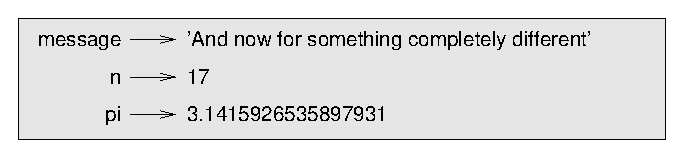
\includegraphics{figs/state2.eps}}
\afterfig

To display the value of a variable, you can use a print statement:

\beforeverb
\begin{verbatim}
>>> print n
17
>>> print pi
3.14159265359
\end{verbatim}
\afterverb
%
The type of a variable is the type of the value it refers to.

\beforeverb
\begin{verbatim}
>>> type(message)
<type 'str'>
>>> type(n)
<type 'int'>
>>> type(pi)
<type 'float'>
\end{verbatim}
\afterverb
%
\begin{exercise}
If you type an integer with a leading zero, you might get
a confusing error:

\beforeverb
\begin{verbatim}
>>> zipcode = 02492
                  ^
SyntaxError: invalid token
\end{verbatim}
\afterverb

Other numbers seem to work, but the results are bizarre:

\beforeverb
\begin{verbatim}
>>> zipcode = 02132
>>> print zipcode
1114
\end{verbatim}
\afterverb

Can you figure out what is going on?  Hint: print the
values {\tt 01}, {\tt 010}, {\tt 0100} and {\tt 01000}.

\index{octal}

\end{exercise}




\section{Variable names and keywords}
\index{keyword}

Programmers generally choose names for their variables that
are meaningful---they document what the variable is used for.

Variable names can be arbitrarily long.  They can contain
both letters and numbers, but they have to begin with a letter.
It is legal to use uppercase letters, but it is a good idea
to begin variable names with a lowercase letter (you'll
see why later).

The underscore character (\verb"_") can appear in a name.
It is often used in names with multiple words, such as
\verb"my_name" or \verb"airspeed_of_unladen_swallow".

\index{underscore character}

If you give a variable an illegal name, you get a syntax error:

\beforeverb
\begin{verbatim}
>>> 76trombones = 'big parade'
SyntaxError: invalid syntax
>>> more@ = 1000000
SyntaxError: invalid syntax
>>> class = 'Advanced Theoretical Zymurgy'
SyntaxError: invalid syntax
\end{verbatim}
\afterverb
%
{\tt 76trombones} is illegal because it does not begin with a letter.
{\tt more@} is illegal because it contains an illegal character, {\tt
@}.  But what's wrong with {\tt class}?

It turns out that {\tt class} is one of Python's {\bf keywords}.  The
interpreter uses keywords to recognize the structure of the program,
and they cannot be used as variable names.

\index{keyword}

Python has 31 keywords\footnote{In Python 3.0, {\tt exec} is no
longer a keyword, but {\tt nonlocal} is.}:

\beforeverb
\begin{verbatim}
and       del       from      not       while    
as        elif      global    or        with     
assert    else      if        pass      yield    
break     except    import    print              
class     exec      in        raise              
continue  finally   is        return             
def       for       lambda    try
\end{verbatim}
\afterverb
%
You might want to keep this list handy.  If the interpreter complains
about one of your variable names and you don't know why, see if it
is on this list.


\section{Statements}

A statement is a unit of code that the Python interpreter can
execute.  We have seen two kinds of statements: print
and assignment.

\index{statement}
\index{interactive mode}
\index{script mode}

When you type a statement in interactive mode, the interpreter
executes it and displays the result, if there is one.

A script usually contains a sequence of statements.  If there
is more than one statement, the results appear one at a time
as the statements execute.

For example, the script

\beforeverb
\begin{verbatim}
print 1
x = 2
print x
\end{verbatim}
\afterverb
%
produces the output

\beforeverb
\begin{verbatim}
1
2
\end{verbatim}
\afterverb
%
The assignment statement produces no output.


\section{Operators and operands}
\index{operator, arithmetic}
\index{arithmetic operator}
\index{operand}
\index{expression}

{\bf Operators} are special symbols that represent computations like
addition and multiplication.  The values the operator is applied to
are called {\bf operands}.

The operators {\tt +}, {\tt -}, {\tt *}, {\tt /} and {\tt **}
perform addition, subtraction, multiplication, division and
exponentiation, as in the following examples:

\beforeverb
\begin{verbatim}
20+32   hour-1   hour*60+minute   minute/60   5**2   (5+9)*(15-7)
\end{verbatim}
\afterverb
%
In some other languages, \verb"^" is used for exponentiation, but
in Python it is a bitwise operator called XOR.  I won't cover
bitwise operators in this book, but you can read about
them at \url{wiki.python.org/moin/BitwiseOperators}.

\index{bitwise operator}
\index{operator!bitwise}

%When a variable name appears in the place of an operand, it
%is replaced with its value before the operation is
%performed.

The division operator might not do what you expect:

\beforeverb
\begin{verbatim}
>>> minute = 59
>>> minute/60
0
\end{verbatim}
\afterverb
%
The value of {\tt minute} is 59, and in conventional arithmetic 59
divided by 60 is 0.98333, not 0.  The reason for the discrepancy is
that Python is performing {\bf floor division}\footnote{In Python 3.0,
the result of this division is a {\tt float}.  The new operator
{\tt //} performs integer division.}.

\index{Python 3.0}
\index{floor division}
\index{floating-point division}
\index{division!floor}
\index{division!floating-point}

When both of the operands are integers, the result is also an
integer; floor division chops off the fraction
part, so in this example it rounds down to zero.

If either of the operands is a floating-point number, Python performs
floating-point division, and the result is a {\tt float}:

\beforeverb
\begin{verbatim}
>>> minute/60.0
0.98333333333333328
\end{verbatim}
\afterverb


\section{Expressions}

An {\bf expression} is a combination of values, variables, and operators.
A value all by itself is considered an expression, and so is
a variable, so the following are all legal expressions
(assuming that the variable {\tt x} has been assigned a value):

\index{expression}
\index{evaluate}

\beforeverb
\begin{verbatim}
17
x
x + 17
\end{verbatim}
\afterverb
%
If you type an expression in interactive mode, the interpreter
{\bf evaluates} it and displays the result:

\beforeverb
\begin{verbatim}
>>> 1 + 1
2
\end{verbatim}
\afterverb
%
But in a script, an expression all by itself doesn't
do anything!  This is a common
source of confusion for beginners.

\begin{exercise}
Type the following statements in the Python interpreter to see
what they do:

\beforeverb
\begin{verbatim}
5
x = 5
x + 1
\end{verbatim}
\afterverb
%
Now put the same statements into a script and run it.  What
is the output?  Modify the script by transforming each
expression into a print statement and then run it again.
\end{exercise}


\section{Order of operations}
\index{order of operations}
\index{rules of precedence}
\index{PEMDAS}

When more than one operator appears in an expression, the order of
evaluation depends on the {\bf rules of precedence}.  For
mathematical operators, Python follows mathematical convention.
The acronym {\bf PEMDAS} is a useful way to
remember the rules:

\index{parentheses!overriding precedence}

\begin{itemize}

\item {\bf P}arentheses have the highest precedence and can be used 
to force an expression to evaluate in the order you want. Since
expressions in parentheses are evaluated first, {\tt 2 * (3-1)} is 4,
and {\tt (1+1)**(5-2)} is 8. You can also use parentheses to make an
expression easier to read, as in {\tt (minute * 100) / 60}, even
if it doesn't change the result.

\item {\bf E}xponentiation has the next highest precedence, so
{\tt 2**1+1} is 3, not 4, and {\tt 3*1**3} is 3, not 27.

\item {\bf M}ultiplication and {\bf D}ivision have the same precedence,
which is higher than {\bf A}ddition and {\bf S}ubtraction, which also
have the same precedence.  So {\tt 2*3-1} is 5, not 4, and
{\tt 6+4/2} is 8, not 5.

\item Operators with the same precedence are evaluated from left to 
right.  So in the expression {\tt degrees / 2 * pi}, the division
happens first and the result is multiplied by {\tt pi}.  
To divide by $2 \pi$, you can use parentheses or write {\tt degrees / 2 / pi}.

\end{itemize}


\section{String operations}
\index{string!operation}
\index{operator!string}

In general, you cannot perform mathematical operations on strings, even
if the strings look like numbers, so the following are illegal:

\beforeverb
\begin{verbatim}
'2'-'1'    'eggs'/'easy'    'third'*'a charm'
\end{verbatim}
\afterverb
%
The {\tt +} operator works with strings, but it
might not do what you expect: it performs
{\bf concatenation}, which means joining the strings by
linking them end-to-end.  For example:

\index{concatenation}

\beforeverb
\begin{verbatim}
first = 'throat'
second = 'warbler'
print first + second
\end{verbatim}
\afterverb
%
The output of this program is {\tt throatwarbler}.

The {\tt *} operator also works on strings; it performs repetition.
For example, \verb"'Spam'*3" is \verb"'SpamSpamSpam'".  If one of the operands
is a string, the other has to be an integer.

This use of {\tt +} and {\tt *} makes sense by
analogy with addition and multiplication.  Just as {\tt 4*3} is
equivalent to {\tt 4+4+4}, we expect \verb"'Spam'*3" to be the same as
\verb"'Spam'+'Spam'+'Spam'", and it is.  On the other hand, there is a
significant way in which string concatenation and repetition are
different from integer addition and multiplication.
Can you think of a property that addition has
that string concatenation does not?

\index{commutativity}


\section{Comments}
\index{comment}

As programs get bigger and more complicated, they get more difficult
to read.  Formal languages are dense, and it is often difficult to
look at a piece of code and figure out what it is doing, or why.

For this reason, it is a good idea to add notes to your programs to explain
in natural language what the program is doing.  These notes are called
{\bf comments}, and they start with the \verb"#" symbol:

\beforeverb
\begin{verbatim}
# compute the percentage of the hour that has elapsed
percentage = (minute * 100) / 60
\end{verbatim}
\afterverb
%
In this case, the comment appears on a line by itself.  You can also put
comments at the end of a line:

\beforeverb
\begin{verbatim}
percentage = (minute * 100) / 60     # percentage of an hour
\end{verbatim}
\afterverb
%
Everything from the {\tt \#} to the end of the line is ignored---it
has no effect on the program.

Comments are most useful when they document non-obvious features of
the code.  It is reasonable to assume that the reader can figure out
{\em what} the code does; it is much more useful to explain {\em why}.

This comment is redundant with the code and useless:

\beforeverb
\begin{verbatim}
v = 5     # assign 5 to v
\end{verbatim}
\afterverb
%
This comment contains useful information that is not in the code:

\beforeverb
\begin{verbatim}
v = 5     # velocity in meters/second. 
\end{verbatim}
\afterverb
%
Good variable names can reduce the need for comments, but
long names can make complex expressions hard to read, so there is
a tradeoff.

\section{Debugging}
\index{debugging}

At this point the syntax error you are most likely to make is
an illegal variable name, like {\tt class} and {\tt yield}, which
are keywords, or \verb"odd~job" and \verb"US$", which contain
illegal characters.

\index{syntax error}
\index{error!syntax}

If you put a space in a variable name, Python thinks it is two
operands without an operator:

\beforeverb
\begin{verbatim}
>>> bad name = 5
SyntaxError: invalid syntax
\end{verbatim}
\afterverb
%
For syntax errors, the error messages don't help much.
The most common messages are {\tt SyntaxError: invalid syntax} and
{\tt SyntaxError: invalid token}, neither of which is very informative.

\index{error message}
\index{use before def}
\index{exception}
\index{runtime error}
\index{error!runtime}

The runtime error you are most likely to make is a ``use before
def;'' that is, trying to use a variable before you have assigned
a value.  This can happen if you spell a variable name wrong:

\beforeverb
\begin{verbatim}
>>> principal = 327.68
>>> interest = principle * rate
NameError: name 'principle' is not defined
\end{verbatim}
\afterverb
%
Variables names are case sensitive, so {\tt LaTeX} is not the
same as {\tt latex}.

\index{case-sensitivity, variable names}
\index{semantic error}
\index{error!semantic}

At this point the most likely cause of a semantic error is
the order of operations.  For example, to evaluate $\frac{1}{2 \pi}$,
you might be tempted to write

\beforeverb
\begin{verbatim}
>>> 1.0 / 2.0 * pi
\end{verbatim}
\afterverb
%
But the division happens first, so you would get $\pi / 2$, which
is not the same thing!  There is no way for Python
to know what you meant to write, so in this case you don't
get an error message; you just get the wrong answer.

\index{order of operations}


\section{Glossary}

\begin{vocabulary}[value:]  One of the basic units of data, like a number or string, 
that a program manipulates.
\index{value}
\end{vocabulary}
	
\begin{vocabulary}[type:] A category of values.  The types we have seen so far
are integers (type {\tt int}), floating-point numbers (type {\tt
float}), and strings (type {\tt str}).
\index{type}
\end{vocabulary}
	
\begin{vocabulary}[integer:] A type that represents whole numbers.
\index{integer}
\end{vocabulary}
	
\begin{vocabulary}[floating-point:] A type that represents numbers with fractional
parts.
\index{floating-point}
\end{vocabulary}
	
\begin{vocabulary}[string:] A type that represents sequences of characters.
\index{string}
\end{vocabulary}
	
\begin{vocabulary}[variable:]  A name that refers to a value.
\index{variable}
\end{vocabulary}
	
\begin{vocabulary}[statement:]  A section of code that represents a command or action.  So
far, the statements we have seen are assignments and print statements.
\index{statement}
\end{vocabulary}
	
\begin{vocabulary}[assignment:]  A statement that assigns a value to a variable.
\index{assignment}
\end{vocabulary}
	
\begin{vocabulary}[state diagram:]  A graphical representation of a set of variables and the
values they refer to.
\index{state diagram}
\end{vocabulary}
	
\begin{vocabulary}[keyword:]  A reserved word that is used by the compiler to parse a
program; you cannot use keywords like {\tt if}, {\tt  def}, and {\tt while} as
variable names.
\index{keyword}
\end{vocabulary}
	
\begin{vocabulary}[operator:]  A special symbol that represents a simple computation like
addition, multiplication, or string concatenation.
\index{operator}
\end{vocabulary}
	
\begin{vocabulary}[operand:]  One of the values on which an operator operates.
\index{operand}

\item[floor division:] The operation that divides two numbers and chops off
the fraction part.
\index{floor division}
\end{vocabulary}
	
\begin{vocabulary}[expression:]  A combination of variables, operators, and values that
represents a single result value.
\index{expression}
\end{vocabulary}
	
\begin{vocabulary}[evaluate:]  To simplify an expression by performing the operations
in order to yield a single value.
\end{vocabulary}
	
\begin{vocabulary}[rules of precedence:]  The set of rules governing the order in which
expressions involving multiple operators and operands are evaluated.
\index{rules of precedence}
\index{precedence}
\end{vocabulary}
	
\begin{vocabulary}[concatenate:]  To join two operands end-to-end.
\index{concatenation}
\end{vocabulary}
	
\begin{vocabulary}[comment:]  Information in a program that is meant for other
programmers (or anyone reading the source code) and has no effect on the
execution of the program.
\index{comment}
\end{vocabulary}
	

\section{Exercises}

\begin{exercise}
Assume that we execute the following assignment statements:

\begin{verbatim}
width = 17
height = 12.0
delimiter = '.'
\end{verbatim}

For each of the following expressions, write the value of the
expression and the type (of the value of the expression).

\begin{enumerate}

\item {\tt width/2}

\item {\tt width/2.0}

\item {\tt height/3}

\item {\tt 1 + 2 * 5}

\item {\tt delimiter * 5}

\end{enumerate}

Use the Python interpreter to check your answers.
\end{exercise}

\begin{exercise}
Practice using the Python interpreter as a calculator: 
\index{calculator}

\begin{enumerate}

\item The volume of a sphere with radius $r$ is $\frac{4}{3} \pi r^3$.
  What is the volume of a sphere with radius 5?  Hint: 392.6 is wrong!

\item Suppose the cover price of a book is \$24.95, but bookstores get a
  40\% discount.  Shipping costs \$3 for the first copy and 75 cents
  for each additional copy.  What is the total wholesale cost for
  60 copies?

\item If I leave my house at 6:52 am and run 1 mile at an easy pace
  (8:15 per mile), then 3 miles at tempo (7:12 per mile) and 1 mile at
  easy pace again, what time do I get home for breakfast?

\index{running pace}

\end{enumerate}
\end{exercise}



%----------------------------------------------------------------------------------------
%	BIBLIOGRAPHY
%----------------------------------------------------------------------------------------

\chapter*{Bibliography}
\addcontentsline{toc}{chapter}{\textcolor{ocre}{Bibliography}}

%------------------------------------------------

\section*{Articles}
\addcontentsline{toc}{section}{Articles}
\printbibliography[heading=bibempty,type=article]

%------------------------------------------------

\section*{Books}
\addcontentsline{toc}{section}{Books}
\printbibliography[heading=bibempty,type=book]

%----------------------------------------------------------------------------------------
%	INDEX
%----------------------------------------------------------------------------------------

\cleardoublepage
\phantomsection
\setlength{\columnsep}{0.75cm}
\addcontentsline{toc}{chapter}{\textcolor{ocre}{Index}}
\printindex

%----------------------------------------------------------------------------------------


\end{document}
